\chapter{Implementation}
\section{Overview}
\quad \ \ Because Halide is not naturally support synergistically computing, we builda framework that execute before calling halide function ,by this execution sequence, we can split works become to two or more parts and dispatch the work to CPU and GPU. Because Halide is a language for image processing, output will be an array.Accoding to the Halide pipeline relations,it's guaranteed that each output will be computed independently and could't be influenced by computing sequence.
With the feature of Halide output, we split output into several sub-blocks by output index and dispatch works by blocks and guarantee that output will be correct.Different from FluidCL, the work assignment of our framework is according to output blocks rather work group in OpenCL.After the execution, we merge the output from different devices become a full result. However Halide is not support this function so we also have to make our framework to receive the output from halide function and merge it and return.

\begin{figure}[!hbtp]
\centering
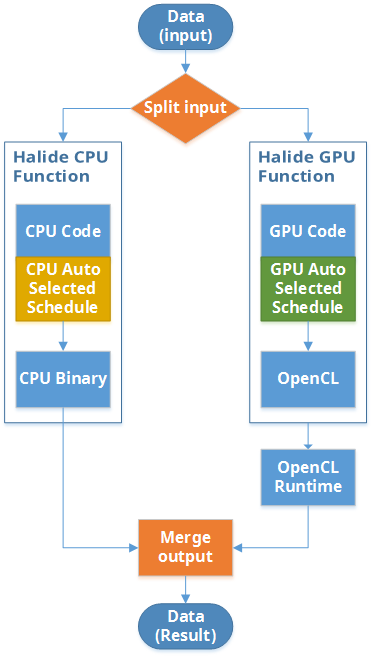
\includegraphics[width=10cm]{img/Framework-SystemFlow.png}
\caption{System Flow}
\label{fig:my_label}
\end{figure}

\begin{figure}[!hbtp]
\centering
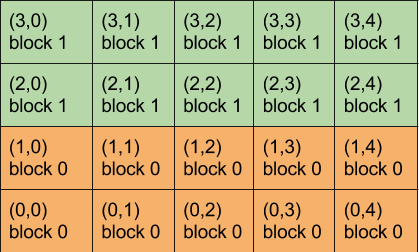
\includegraphics[width=10cm]{img/show_blocks.png}
\caption{Output nubmering.Each elements of output array is shown as a tuple(x,y) with x and y being row and column idex,The number shown in boldface is the block id}
\label{fig:my_label}
\end{figure}

\section{Buffer setup}
\quad \ \ In default way, the Halide will allocate a whole new space in main memory for storage output. If execution device is CPU, output will directly write into the main memory space. However, if the execution device is GPU, Halide will first copy the input main memory to GPU memory. After finishing the computing, Halide will copy the output from GPU memory to main memory. And we have to copy the output from GPU into a new memory space to fit the buffer format of Halide which is shown as Figure ~\ref{fig:Halide_default}. That is, if we use Halide default way to manage memory we have to do memory copy three times (From main memory to GPU, From GPU memory to main memory and from main memory to other main memory spcae to merge output) shown as Figure ~\ref{fig:Halide_default1}.To solve this problem, we have to take over the memory management from Halide by allocating a full size memory and setting the stride for it. In detail, when we  allocate a Halide buffer, it will automatically call a function by Halide to setup the dimensions, boundary and stide for each dimension and create a array as a buffer to save to data. When using our framework we will allocation new buffers for each device, calculate the corresponding boundary and stride for new buffers and set the memory address of the array of the new output buffer to the address of the array of original output buffer which is passed by programmer(Figure ~\ref{fig:memory_new}). By this way, after GPU finish its work, the result can directly copy to the main memory at correctly position.




\begin{figure}[!hbtp]
\centering

\includegraphics[width=10cm]{img/memory_full.png}
\caption{Original Halide output format}
\label{fig:Halide_default}
\end{figure}

\begin{figure}[!hbtp]
\centering
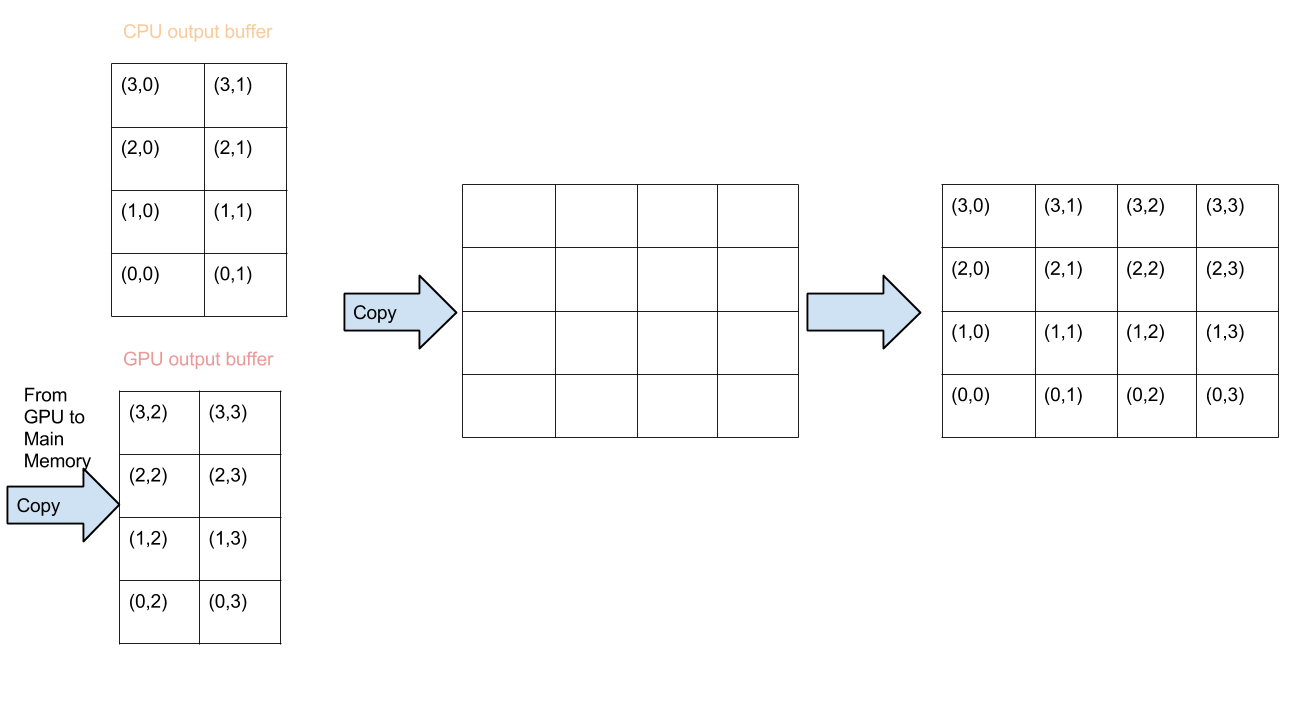
\includegraphics[width=10cm]{img/Memory_copy.png}
\caption{Original Halide output merging}
\label{fig:Halide_default1}
\end{figure}

\begin{figure}[!hbtp]
\centering
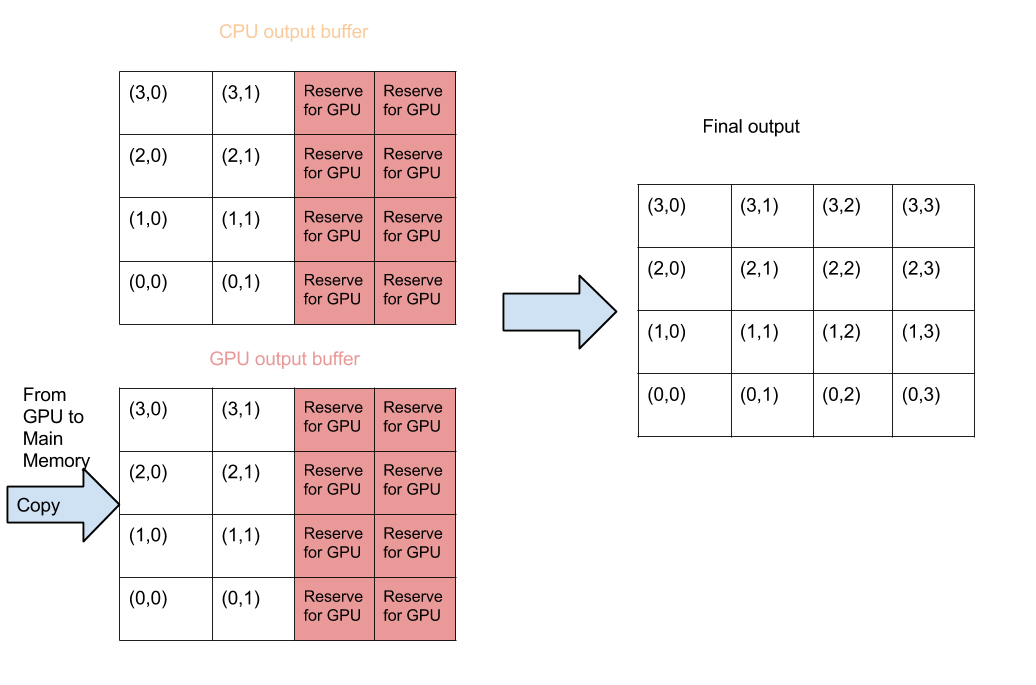
\includegraphics[width=10cm]{img/Memory_copy_new.png}
\caption{Buffer with reserving space}
\label{fig:memory_new}
\end{figure}



\section{Static Dispatch}
\quad\ \ After solving the redundant memory copy problem, we were trying to implement a simple method to achieve the goal that synergistically computing .When the framework is used with specifically workload, we will prepare the output space and set the output stride and other argument by referencing the workload for each CPU and GPU Halide function.  After setting the output for each Halide function, we call Halide function with full size input and the output pointer we prepared for each devices with two thread, one for CPU function and one for GPU. When GPU finished jobs, the output is still kept in GPU memory, the framework should call the function which is provided by Halide to copy the result from GPU memory to main memory. After both CPU and GPU work threads are completed, we will return the final result to the caller. With this implementation, we got about 50\% speedup, the detail experiment result will be shown in next Chapter.

% Furthermore, we implement work stealing skill to speedup static way. By this implementation, we split the workload of CPU into N blocks from 0 to N-1 and the workload of GPU still keep as one block. The CPU thread process blocks sequentially. After GPU finished its workload, The GPU thread will check the status of blocks from N-1 to 0 which should belong to CPU, if there is a block have not been done, GPU will help to process the block. The workload stealing can improve 8\% more compared to static way.

\begin{figure}[hbtp]
\centering
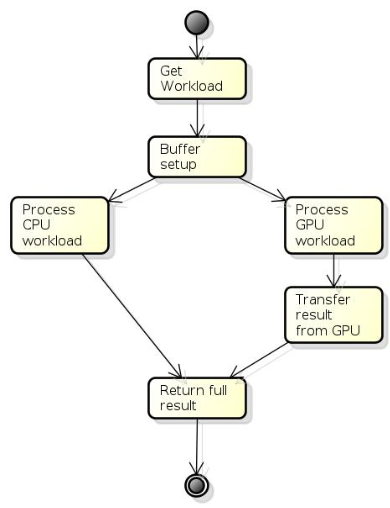
\includegraphics[height=10cm]{img/StaticDispatch.png}
\caption{Flowchart of Static Dispatch}
\label{fig:my_label}
\end{figure}

\section{Dynamic Dispatch}

\quad \ \ By the implementation above, we create an environment to split computation into CPU part and GPU part. However, the decision of the workload on different devices is still  a problem to programmer ,in addition, to get better workload still need an offline profiler to profile the computation. To solve this problem, we implemented a runtime system to manage the workload by split the output into N blocks from 0 to N-1.we let CPU process blocks in increasing order and GPU process blocks from the other end. By this order, CPU and GPU will execute without overlapping.

	To achieve this implementation, we maintain a status table to record the status of each block. When CPU start to process a block, the runtime of CPU part will check the block status is empty or not .If it is empty, it change the status of the block from empty to computing, otherwise, it will stop the computation of CPU part. And CPU runtime will set the parameter and call halide CPU function. After Halide CPU function finished a block, Halide function will directly write the result into output buffer we prepared and the CPU runtime will change the status of the block to finished and process next block. When GPU runtime is going to process a block, it will also check the status of the block like CPU runtime, only when the status of the block is empty, GPU would process the block. When working thread is going to process to the block which is processed by and other devices, the work thread will be terminated by checking the status of next block, that is, if the status of next target block is not empty which means the other part of work is done by another device, the work thread will be terminated. After both work thread finished its jobs, we will return the final result to the caller.
\begin{figure}[hbtp]
\centering
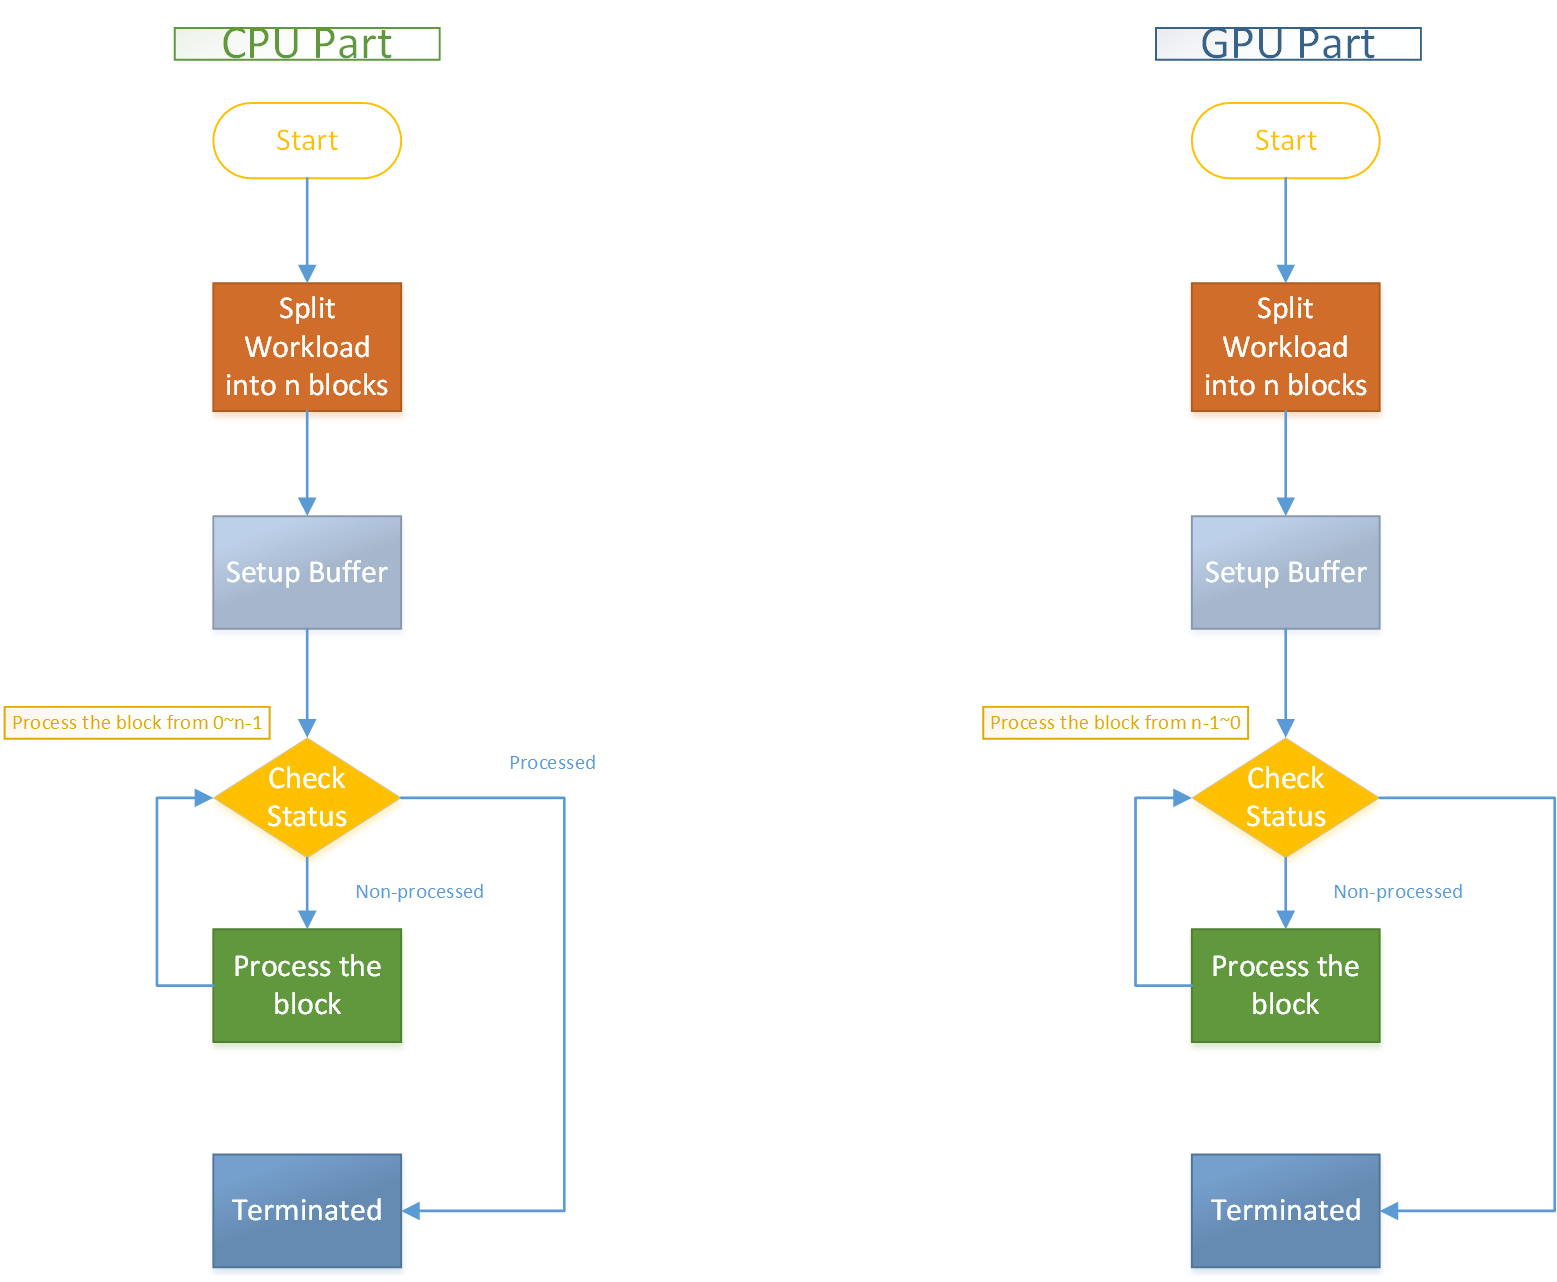
\includegraphics[height=10cm]{img/DynamicDispatchFlow.png}
\caption{Flowchart of Dynamic Dispatch}
\label{fig:my_label}
\end{figure}

\section{Usage of our framework}
\quad \ \ In native Halide, we will get extern functions for different processor which is generated by Halide AOT compiler and will call the function with parameters for the algorithm, input buffer and output buffer in another c++ source file.Here is an example below.
\lstset{language=C++} % Set your language (you can change the language for each code-block optionally)
\begin{lstlisting}[frame=single] % Start your code-block 
//Halide Function
local_laplacian_gpu(levels,alpha/(levels-1),beta,
	input,output); //Halide GPU Function
local_laplacian_cpu(levels,alpha/(levels-1),beta,
	input,output); //Halide CPU Function
\end{lstlisting}

To our framework, you just need to declare a object named StaticDispatch or DynamicDispatch and pass input and output buffer to its constructor.When you want to compute the result just call the function named realize with Halide CPU function, Halide GPU function, workload(if you are using static dispatch), parameters for the algorithm.There are example for using static dispatch and dynamic dispatch below.
\lstset{language=C++} % Set your language (you can change the language for each code-block optionally)
\begin{lstlisting}[frame=single] % Start your code-block 
//Static Dispatch
StaticDispatch static(input,output);
static.realize(local_laplacian_cpu,local_laplacian_gpu,
	workload,levels,alpha/(levels-1),beta);
\end{lstlisting}
\lstset{language=C++} % Set your language (you can change the language for each code-block optionally)
\begin{lstlisting}[frame=single] % Start your code-block 
//Dynamic Dispatch
DynamicDispatch dynamic(input,output);
dynamic.realize(local_laplacian_cpu,local_laplacian_gpu,
	levels,alpha/(levels-1),beta);
\end{lstlisting}
